%!TEX root=../robocert.tex
\begin{figure}
	\centering
	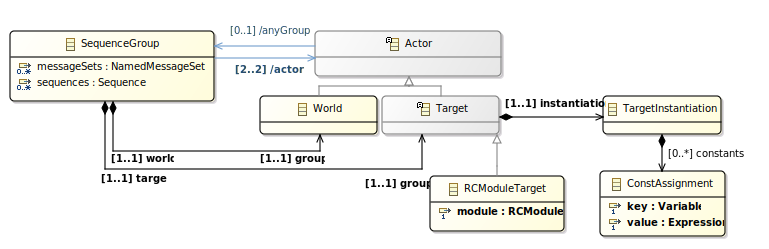
\includegraphics[width=\textwidth]{diagrams/Actors}
	\caption{Class diagram for the part of the \langname{} metamodel dealing with actors.}
	\label{fig:metamodel-actors}
\end{figure}

\Cref{fig:metamodel-actors} depicts the part of the metamodel concerning
actors.

\subsection{\mactor}

An \mactor{} is a named participant in a sequence.  The names can be used to
specify the source and recipient of communications in \mmessagespec{}s.
As mentioned in
\cref{sec:metamodel-sequences}, there are always two actors
attached to a sequence: a \mtarget{} (\cref{ssec:metamodel-actors-target})
and a \mworld{} (\cref{ssec:metamodel-actors-world}).

\subsection{\mtarget}\label{ssec:metamodel-actors-target}

A \mtarget{} references the part of a robotic system that serves as the focus
for a particular sequence diagram.  There is
presently one type of target, with more to appear later:

\begin{itemize}
\item
	a \mrcmoduletarget{} references a \mrcmodule.
\end{itemize}

All forms of \mtarget{} contain a \mtargetinstantiation{} (see below), which
is always applied to any use of that target; assertions may further instantiate
any constants left open by the target's \mtargetinstantiation.

\begin{lstlisting}[style=Example]
module AModule as M
// RCModuleTarget with implicit empty TargetInstantiation

module AModule
    with { SOME_CONSTANT set to 4, ANOTHER_CONSTANT set to 5 }
    as M
// RCModuleTarget with explicit TargetInstantiation
\end{lstlisting}

\subsection{\mtargetinstantiation}

A \mtargetinstantiation{} instantiates some or all of the constants in the
target's parametrisation.  It contains a list of key/value pairs where each key
is a RoboChart \mvariable{} corresponding to a constant, and each value is a
RoboChart \mexpression{} evaluated in an arbitrary \todo{check this} scope.

\begin{lstlisting}[style=Example]
{ SOME_CONSTANT set to 4, ANOTHER_CONSTANT set to 5 }
\end{lstlisting}

\subsection{\mworld}\label{ssec:metamodel-actors-world}

A \mworld{} is an \mactor{} that represents the `world' outside a sequence's
\mtarget.  \mworld s do not contain any data.

\begin{lstlisting}[style=Example]
world as W
\end{lstlisting}

%%% Local Variables:
%%% mode: latex
%%% TeX-master: "../robocert"
%%% End:
